%!TEX root = ../dissertation.tex

\Chapter{Supplementary information for Chapter~\ref{sec:memory}}

\section{Deviations from pre-registration}\label{app:deviation}

After pre-registering and running the experiments, we discovered a flaw in the implementation of the lesioned models without meta-level control. In our first implementation, stopping times and fixation durations were sampled directly from the empirical distribution in the human data (discretized into 100ms time steps). We reasoned that this would give the model the best chance of capturing the human behavior without a metacognitive component. However, we later realized that this approach effectively prevents the model from utilizing non-decision time, as any non-decision time would be added to a distribution that already perfectly matches the human data.

After realizing this, we implemented the more flexible lesioned model with stopping times and fixation durations drawn from arbitrary Gamma distributions, as reported in the main text. Note that this model has more free parameters in the two-item case, thus we also decide to fit the lesioned model to data in Experiment 2 (contrary to our intention to use the fitted parameters from Experiment 1). The predictions of the original model for both experiments are shown in Figures~\ref{fig:exp1_rt_alt}-\ref{fig:commitment_alt}.

This analysis also revealed that two of the effects which we had believed to be evidence of meta-level control could in fact be produced by the model without meta-level control. The first such effect is shown in Figure~\ref{fig:exp1_cum}B. The original logic of this plot was to look at how strength affects the decision to skip a trial over time, after factoring out the indirect effect of strength on recall (which in turn prevents skipping). With a low or moderate non-decision time distribution, this effect cannot be captured by a model without meta-level control (as can be seen in the plot). However, when non-decision time is a sufficiently large portion of total response time, the effect can be produced through mechanistic means. Given this, we could not provide a useful interpretation of the effect, and thus removed it from the main text.

The second effect is the prediction that final fixations are longer than non-final fixations (Figure~\ref{fig:commitment}A). We elected to keep this effect in the main text because its interpretation as an indication of rational metamemory was further supported by the additional analysis of the distribution of pretest accuracy for long fixations (Figure~\ref{fig:commitment}B).

\begin{figure}[]
  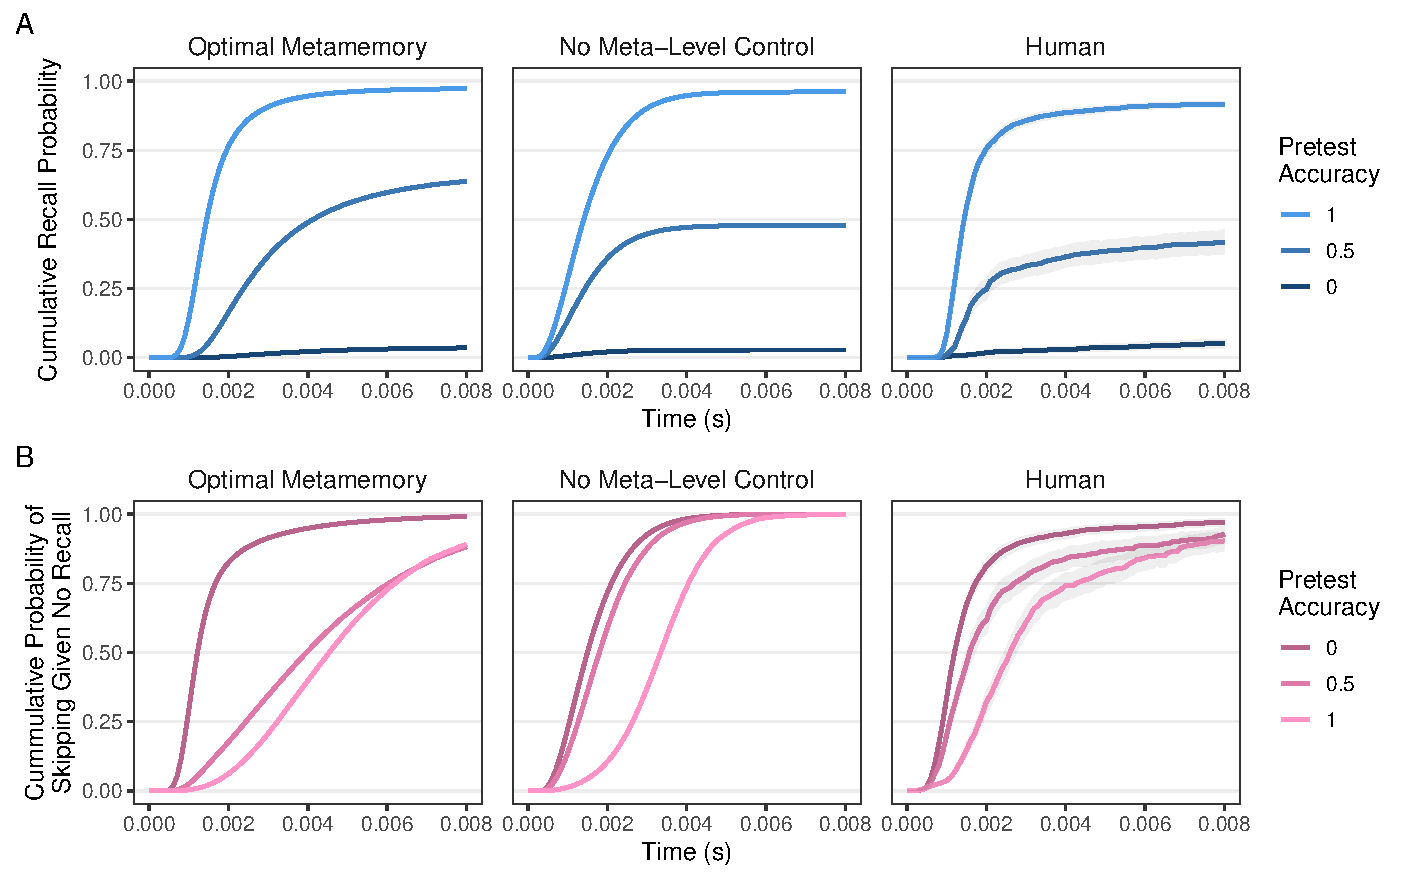
\includegraphics[scale=.65]{figs/memory/exp1/cum_probs.pdf}
  \caption{%
    Timecourse of recall and stopping.
    (A) For each time point (in 100ms steps), the proportion of trials on which the target was recalled before that point, grouping trials by the accuracy rate of the presented cue in the pretest phase.
    (B) For each time point, the proportion of trials that were skipped before that point, conditioning on the fact that the target had not already been recalled.
    \emph{Note}: Lines show means of participants means and ribbons show 95\% bootstrapped confidence intervals over participant means.
  }
  \label{fig:exp1_cum}
\end{figure}


\begin{figure}[]
  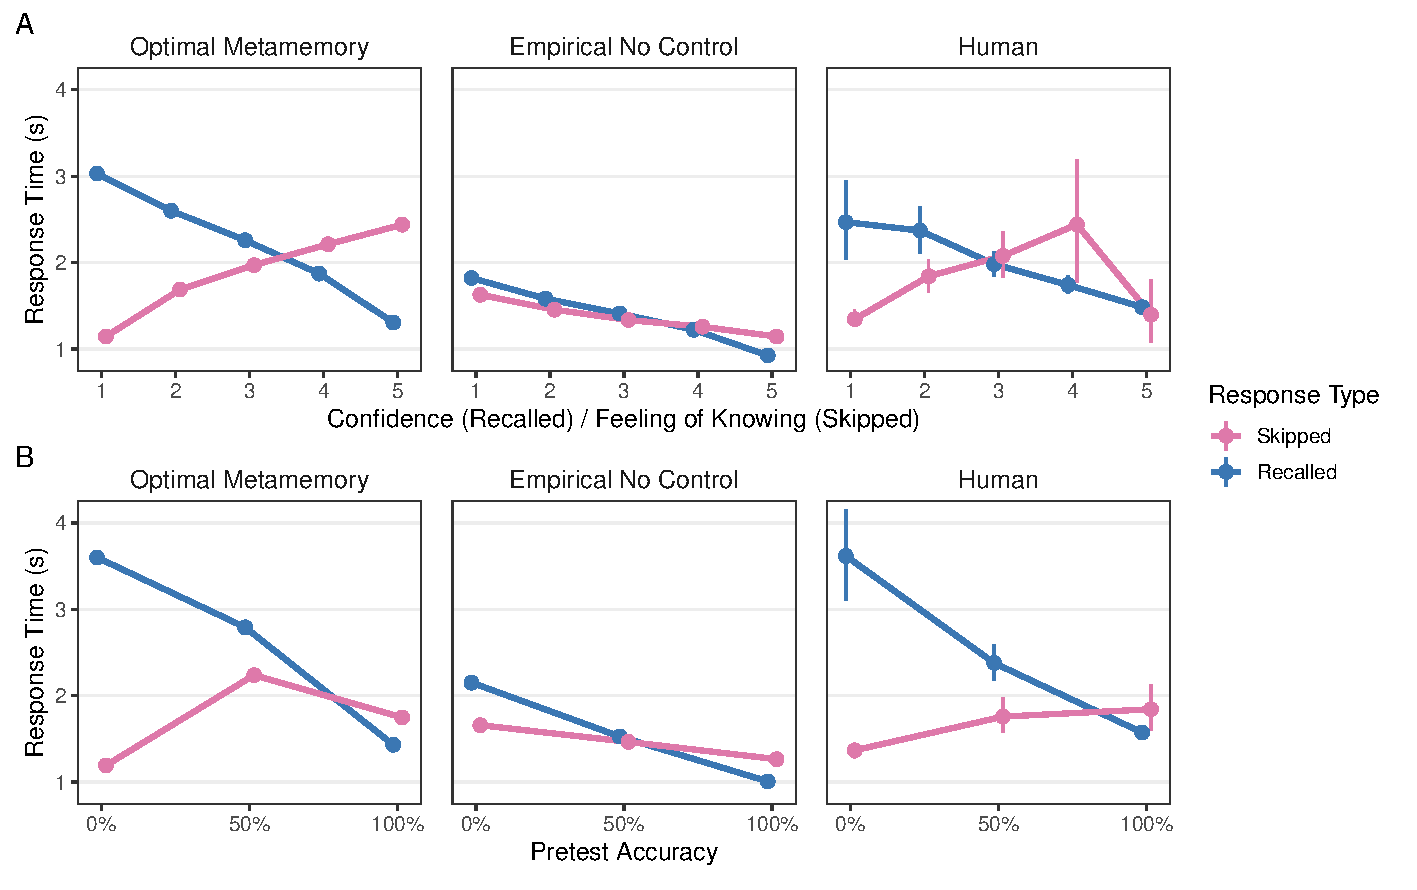
\includegraphics[scale=.65]{figs/memory/exp1_alt/rt.pdf}
  \caption{Alternative version of Figure~\ref{fig:exp1_rt} where the lesioned model draws stopping times from the empirical distribution.}
  \label{fig:exp1_rt_alt}
\end{figure}

\begin{figure}[ht]
  \centering
  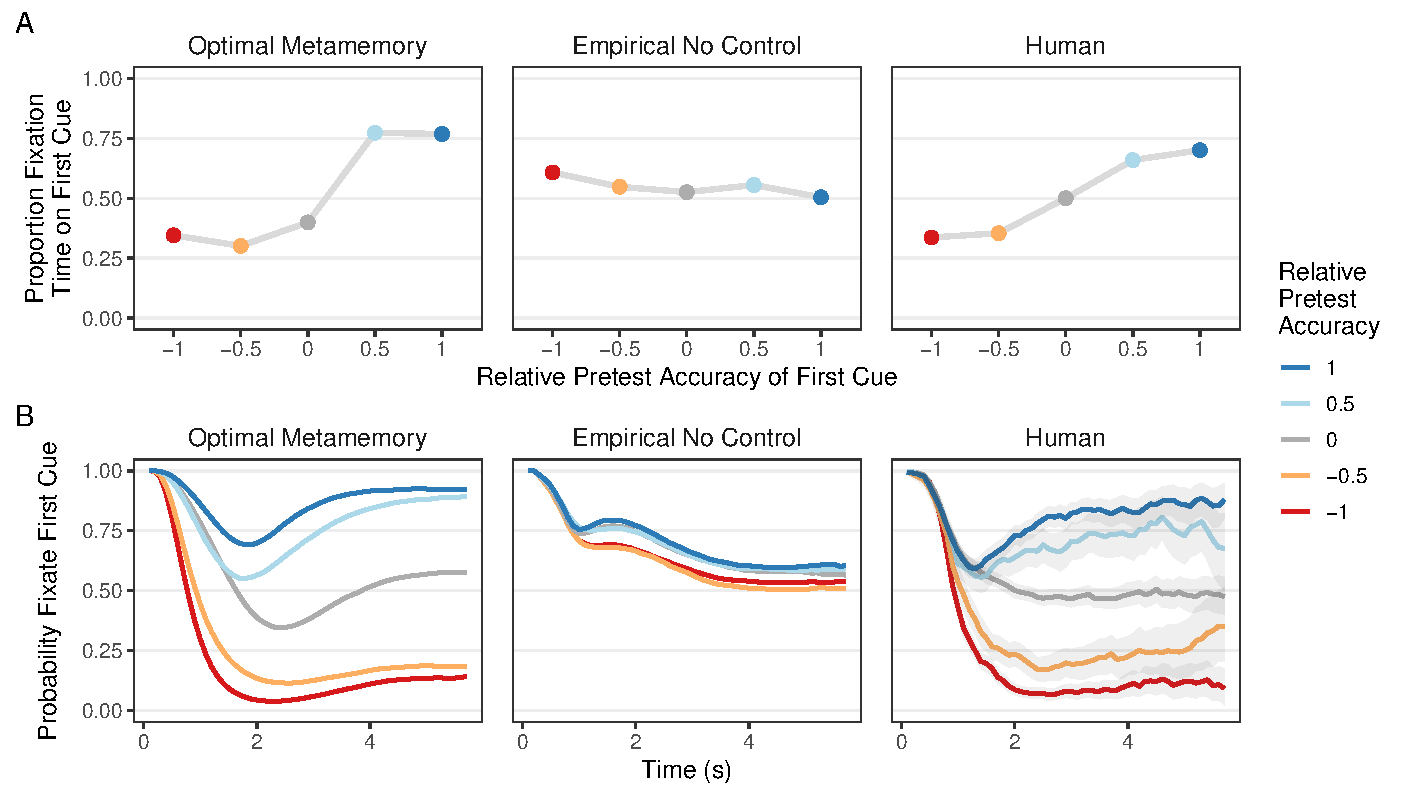
\includegraphics[scale=.65]{figs/memory/exp2_alt/overall_timecourse.pdf}
  \caption{Alternative version of Figure~\ref{fig:timecourse} where the lesioned model draws stopping and switching times from the empirical distribution.}
  \label{fig:timecourse_alt}
\end{figure}

\begin{figure}[t]
  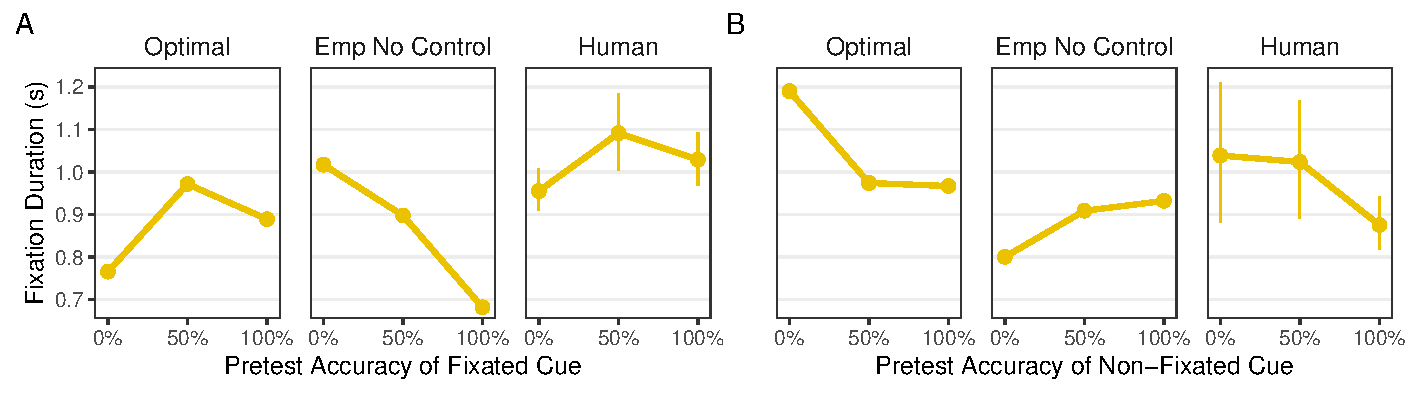
\includegraphics[scale=.65]{figs/memory/exp2_alt/fixation_durations.pdf}
  \caption{Alternative version of Figure~\ref{fig:nonfinal} where lesioned model draws stopping and switching times from the empirical distribution.}
  \label{fig:nonfinal_alt}
\end{figure}

\begin{figure}[t]
  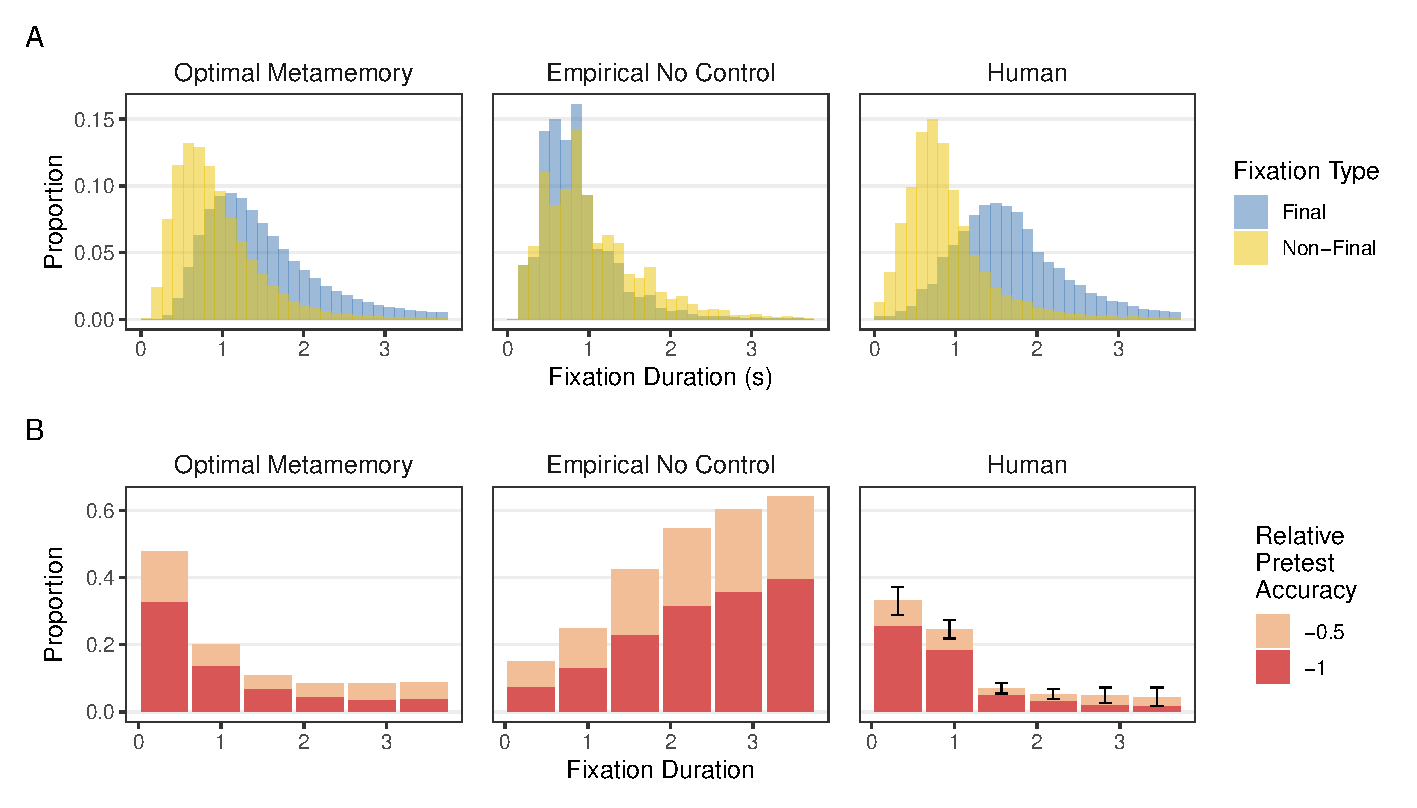
\includegraphics[scale=.65]{figs/memory/exp2_alt/commitment.pdf}
  \caption{Alternative version of Figure~\ref{fig:commitment} where lesioned model draws stopping and switching times from the empirical distribution.}
  \label{fig:commitment_alt}
\end{figure}


\section{Optimizing the lesioned model to predict effects}\label{app:lesion-search}

To more conclusively determine which effects are inconsistent with the lesioned model, we conducted a thorough search of the parameter space to see if the model could produce each qualitative effect under any parameter setting. For each experiment, we sampled 100,000 parameter configurations and simulated 100,000 trials for each. From these, we excluded simulations with accuracy below 1\% or above 99\%, as these yield unreliable estimates for effects that condition on accuracy. For similar reasons, in Experiment~2, we excluded configurations for which fewer than 1\% of trials had at least two fixations. For each unexcluded simulation, we then performed a standard linear regression corresponding to the regression we reported in the main text. Next, we selected the 100 configurations who produced the largest effect, as estimated by the lower bound of a 95\% confidence interval (this prevents selecting for models that simply produce highly variable estimates). If the lower confidence bound for any of these was larger than a ``minimal interesting difference'', then we concluded that the lesioned model could produce the effect.

\subsection{Experiment 1}

As expected, we found that the lesioned model could predict the observed negative relationship between both judgments and pretest accuracy on response time for the correct trials. Surprisingly, we also found that the lesioned model could predict a substantial positive relationship between judgment and response time on the skip trials (B = -1.925; 95\% CI [-1.93, -1.92]; $B$ is in units of seconds over pretest accuracy, as in the main text). However, this model failed to predict the negative relationship on correct trials (B = -0.761; 95\% CI [-0.762, -0.76]; note that $B$ should be negative). No parameter configuration was able to predict the crossover pattern, with a negative relationship between judgment and response time on correct trials but a positive relationship on skip trials. Furthermore, no configuration was able to predict the positive relationship between pretest accuracy and response time on skip trials (even allowing the relationship for correct trials to be positive).

\subsection{Experiment 2}

The more stringent 65\% requirement (compared to 84\% in the human data) ensures that the model cannot capture the effect through a strong selection effect that was not present in the human data. Consistent with Figures~\ref{fig:timecourse}A and~\ref{fig:commitment}A, the lesioned model was able to capture the overall-proportion and the long-final-fixation effects.

Perhaps surprisingly, we found that the lesioned model was also capable of capturing the both fixation duration effects (fixated: B = 0.11; 95\% CI [0.104, 0.117]; non-fixated: B = 0.095; 95\% CI [0.087, 0.102]). However this configuration (which, not coincidentally, maximized both effects) achieved an accurracy of only 7.3\%. The model was able to capture the effect through a selection effect. It only provided a correct response on the small percentage of trials in which it happened to sample long fixations on the strongest cues. Running the analysis again with the requirement that the model achieve at least 65\% accuracy (compared to 84\% in the human data), we found that no configuration could capture the non-final fixation duration effects.
